
\begin{frame}
  \frametitle{Évolution des Processeurs Graphiques}
  \begin{center}
    \begin{tikzpicture}[yscale=-1]
      % \draw[help lines] (0,0) grid (15,6);
      % > latex arroxw
      \draw[line width=10pt,-latex] (1.5,1) .. controls +(1,4) and +(-5,-0) .. +(10,4);
      \node at (1.5,1) {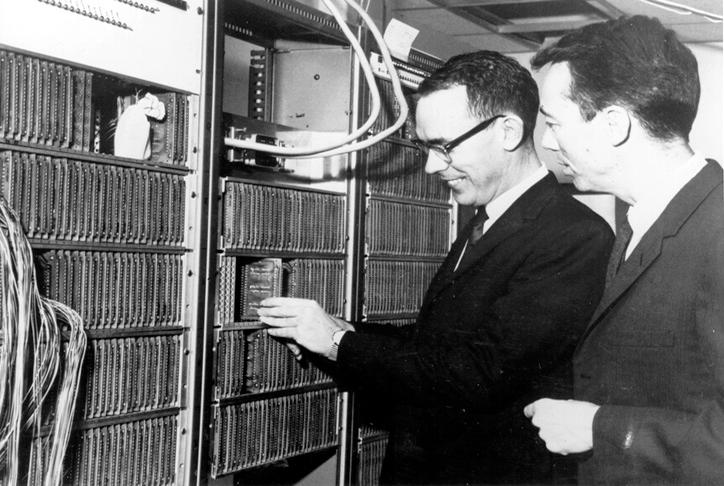
\includegraphics[scale=.1]{images/evans-sutherland.jpg}};
      \node [anchor=south] at (1.5,0) {Evan \& Sutherland};
      \node at (3,3.25) {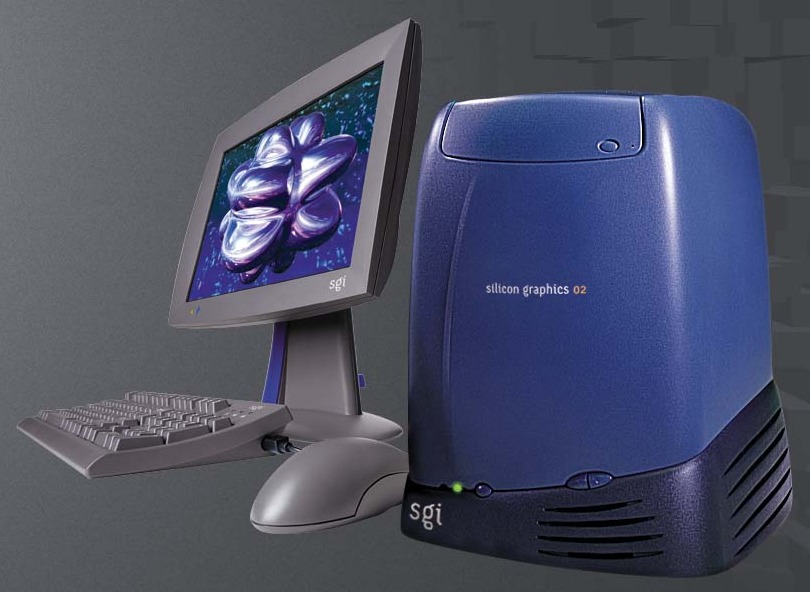
\includegraphics[scale=.1]{images/sgi-o2-workstation.jpg}};
      \node [anchor=north] at (2.5,4.25) {SGI Workstation};
      \node at (6,4.75) {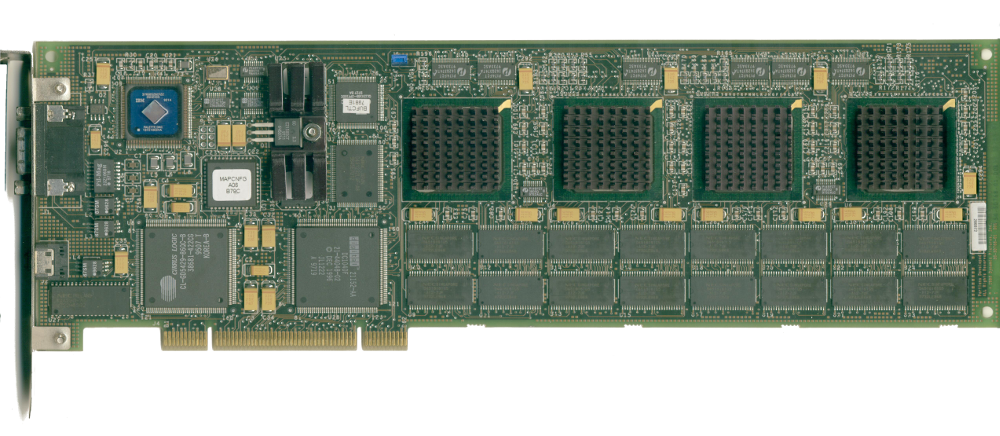
\includegraphics[scale=.5]{images/oxygen.png}};
      \node [anchor=north] at (6,5.25) {Accélerateur Graphique};
      \node at (9,5) {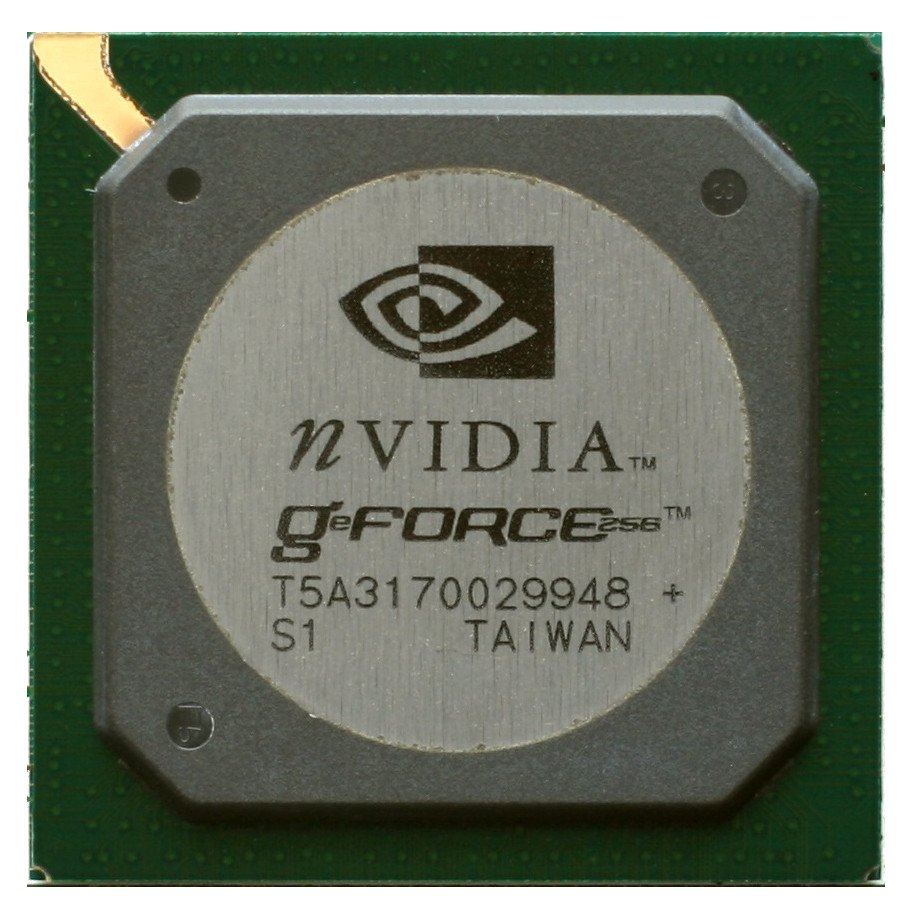
\includegraphics[scale=.03]{images/nvidia-gforce.png}};
      \node [anchor=south,align=center] at (9,4.5) {Nvidia GeForce 256\\ $1^\text{er}$ GPU};
      \node [anchor=west,align=left] at (11.5,5) {\textbf{General Purpose} \\ \textbf{GPU}};
      \draw (14.5,0) -- +(.01,0); % hack
    \end{tikzpicture}
  \end{center}
  \begin{textblock}{12}(5,2)
    \textbf{Convergence}
    \begin{itemize}
    \item du hardware professionnel et grand-publique
    \item des processeurs graphiques et de flux
    \item des plateformes~: de l'embarqué au super-calculateur 
    \end{itemize}
  \end{textblock}
 \end{frame}

\begin{frame}
  \frametitle{Présentation des GPUs~: processeur de flux}
  % dessin flux de données traversant la page
  \begin{center}
    \begin{tabular}{cc}
      Intel Haswell Die & Nvidia Kepler Die \\[5mm]
      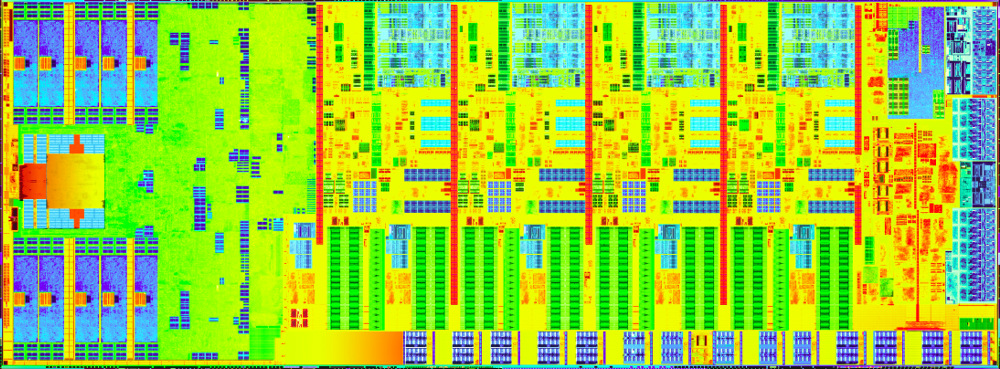
\includegraphics[height=.3\textheight]{images/intel-haswell-die.jpg} &
      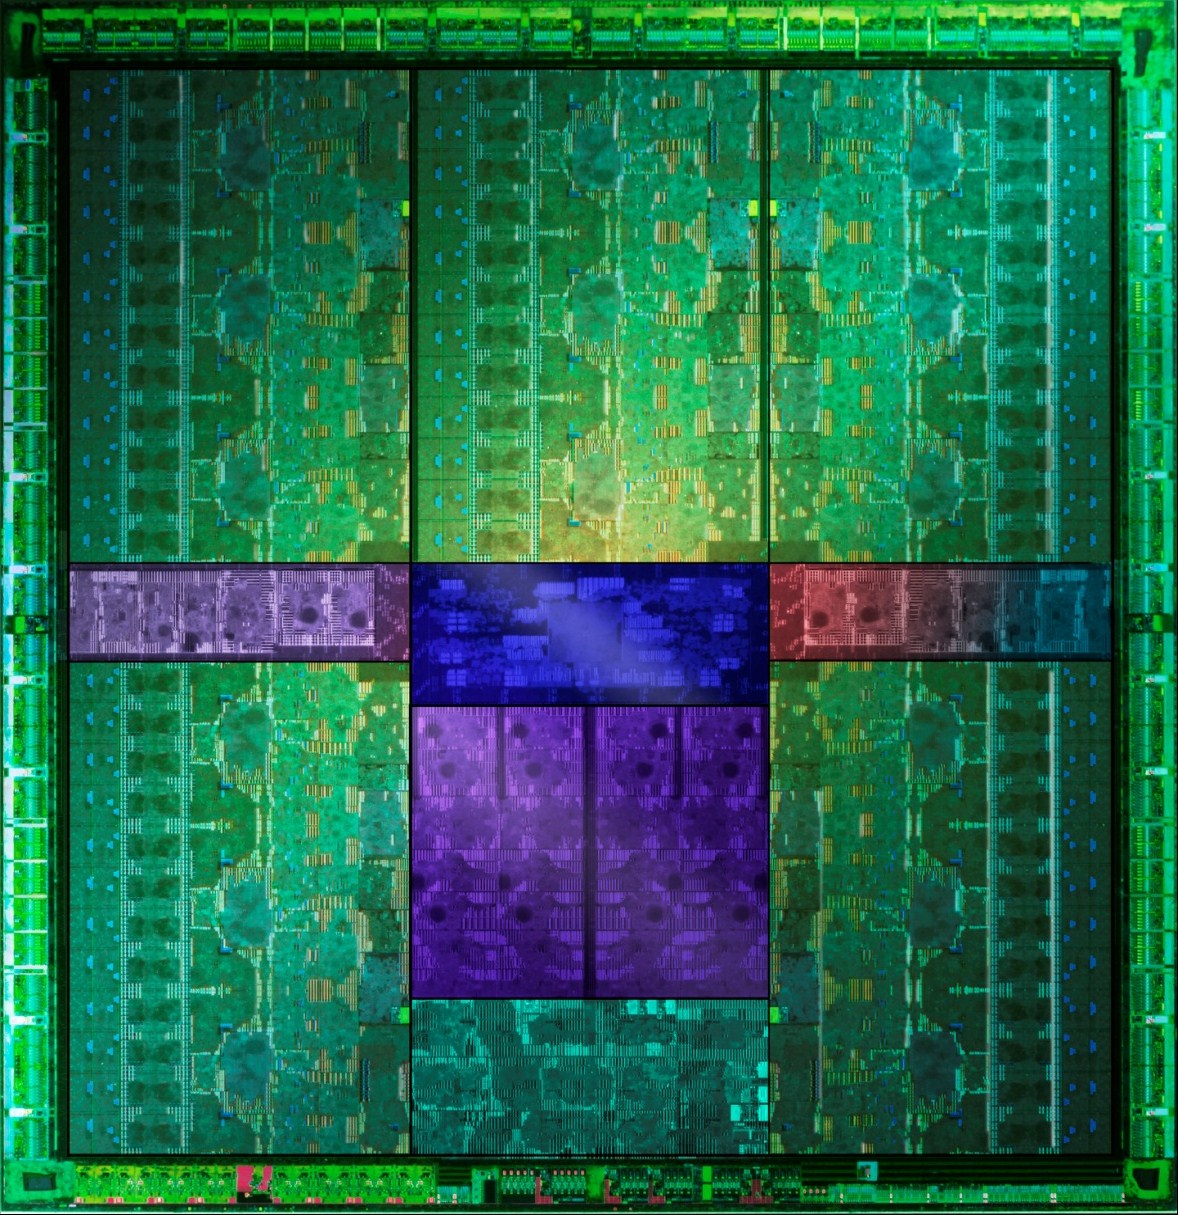
\includegraphics[height=.3\textheight]{images/nvidia-kepler-die.jpg}
    \end{tabular} \\[5mm]
    Architecture de calcule hautement parallèle \\
    couplé à une mémoire rapide (GDDR5)
  \end{center}
  \note[enumerate]
  {
  \item CPU~: usage générique
  \item SIMD AVX2 256-bit 8x float 32-bit
  }
\end{frame}

\begin{frame}
  \frametitle{Usage des GPUs}
  % keywords picture
  % pgf mindmap cf. p75
  % image android qml dans le coin
  \begin{columns}
    \begin{column}{.25\textwidth}
      \begin{center}
        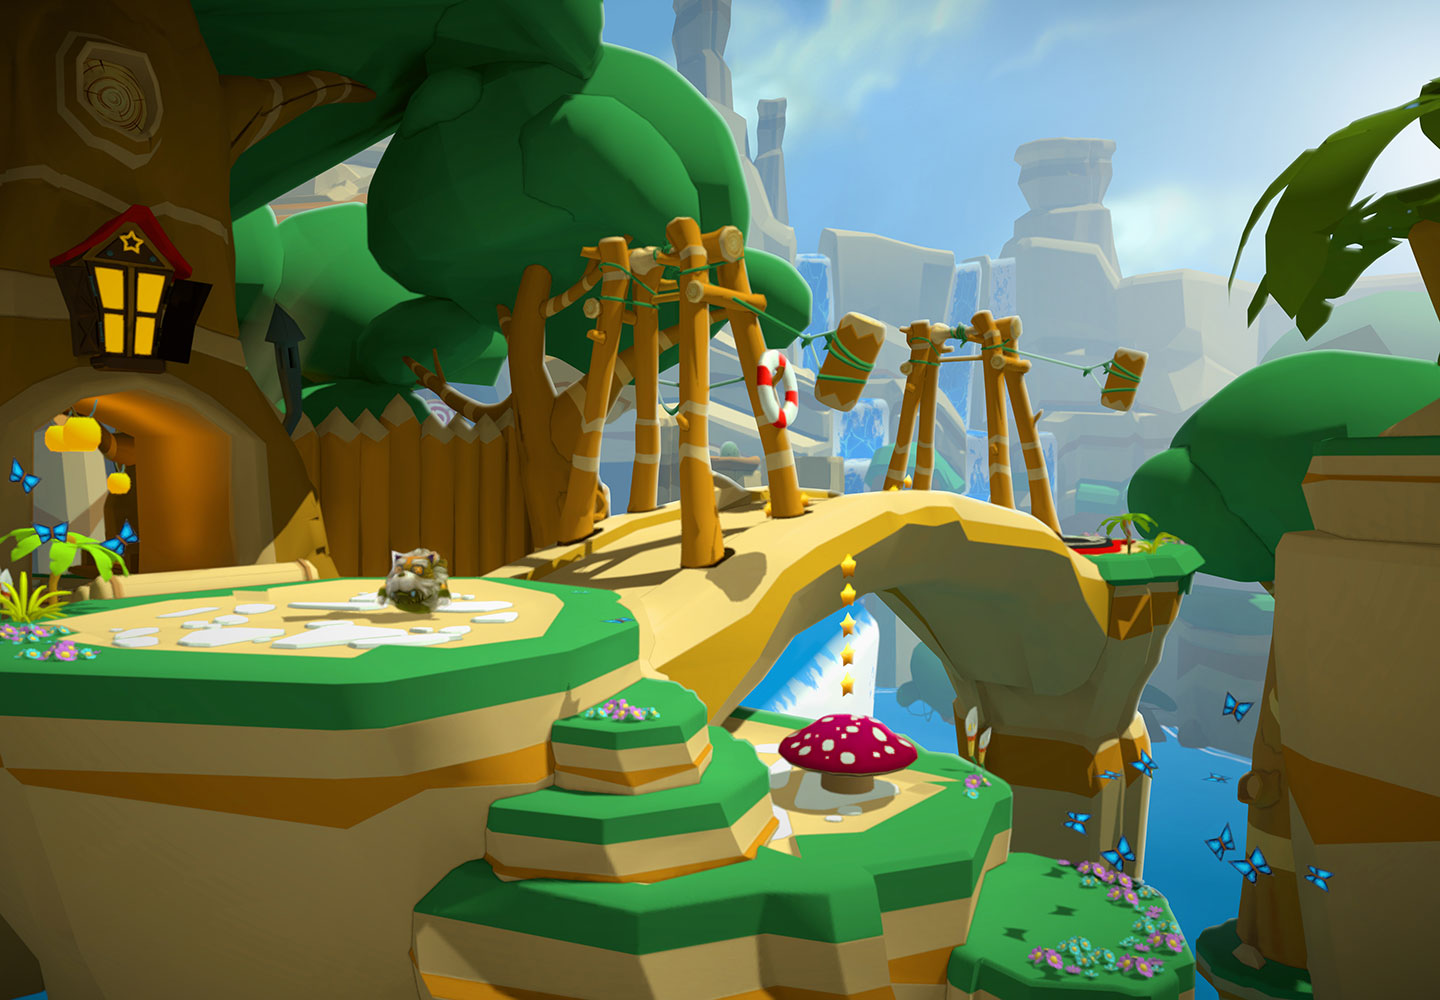
\includegraphics[width=1.\textwidth]{images/game.jpg} \\[5mm]
        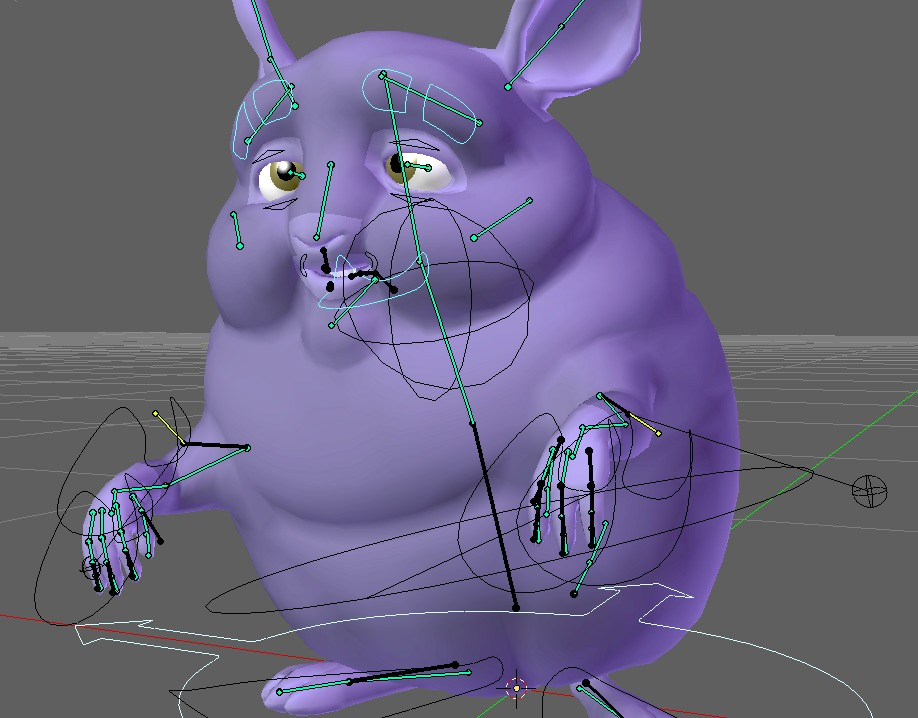
\includegraphics[width=1.\textwidth]{images/blender.jpg}
      \end{center}
    \end{column}
    \begin{column}{.25\textwidth}
      \begin{center}
        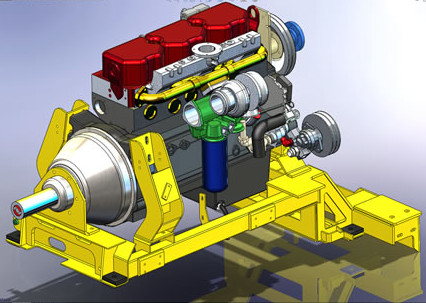
\includegraphics[width=1.\textwidth]{images/solidworks.jpg} \\[5mm]
        
\includegraphics[width=.8\textwidth]{images/tiger.jpg}
      \end{center}
    \end{column}
    \begin{column}{.5\textwidth}
      \begin{itemize}
      \item Moteur de jeu % Game Engine
      \item Modeleur \textbf{3D}
      \item CAO
      \item \textbf{Visualisation} scientifique
      \item \textbf{Interface graphique} \\
        e.g.\ Qt QML, KDE Plasma
      \item \textbf{2D} avec accélération matériel
      \item \textbf{Calcul}~: CUDA, OpenCL
      \end{itemize}
    \end{column}
  \end{columns}
  \note[enumerate]
  {
  \item \url{https://developer.nvidia.com/nv-path-rendering} \\
    KILGARD, M., AND BOLZ, J. 2012. GPU-accelerated path rendering. ACM Transactions on Graphics
    (Proceedings of SIGGRAPH Asia 2012) 31, 6. 106
  \item Shader-based Antialiased Dashed Stroked Polylines \\
    N. P. Rougier. Journal of Computer Graphics Techniques, 2.2 (2013). \\
    \url{http://jcgt.org/published/0002/02/08/}
  \item Higher Quality 2D Text Rendering \\
    N. P. Rougier. Journal of Computer Graphics Techniques, 2.1 (2013). \\
    \url{http://jcgt.org/published/0002/01/04/}
  \item OpenVG, SVG, Display Postscript
  }
\end{frame}

\begin{frame}
  \frametitle{Présentation de l'API OpenGL}
  % même titre que ...
  \begin{columns}
    \begin{column}{.2\textwidth}
      \begin{center}
        
\includegraphics[width=1.\textwidth]{images/khronos-logos/OpenGL/OpenGL_500.jpg} \\
        
\includegraphics[width=1.\textwidth]{images/khronos-logos/OpenGL_ES/OpenGL-ES_500.jpg} \\
        
\includegraphics[width=1.\textwidth]{images/khronos-logos/WebGL/WebGL_500.jpg} \\
        
\includegraphics[width=1.\textwidth]{images/khronos-logos/Khronos_Group/Khronos_Group_500.jpg}
      \end{center}
    \end{column}
    \begin{column}{.8\textwidth}
      \begin{itemize}
        \item Un standard \textbf{ouvert} piloté par le groupe Khronos
        \item La seule API \textbf{cross-platforme} et \textbf{cross-vendor} % cross / multi
        \item L'API de facto de GNU/Linux et d'Android
        \item Une API orientée desktop (OpenGL) et embarqué (OpenGL ES)
        \item mais aussi orientée web (WebGL)
      \end{itemize}
    \end{column}
  \end{columns}
\end{frame}

\begin{frame}
  \frametitle{Évolution de l'API OpenGL}
  \begin{center}
    \includegraphics[width=.6\textwidth]{figures/opengl-release-date.pdf} % ,transparent
  \end{center}
  \note[enumerate]
  {
  \item 20 ans
  \item dynamique des releases
  }
\end{frame}

\begin{frame}
  \frametitle{Programmable Pipeline}
\end{frame}

\begin{frame}
  \frametitle{Implémentations}
  \begin{center}
    \includegraphics[width=.6\textwidth]{figures/mesa-status.pdf} % ,transparent
  \end{center}
\end{frame}

\begin{frame}
  \frametitle{Outils pour interfacer du code C avec Python}
  \begin{center}
    % \begin{tabular}{|c|c|c|}
    \begin{tabular}{ccc}
      & Avantages & Inconvénients \\[.5em]
      %
      API C Python &
      \begin{minipage}[t]{.2\linewidth}
        \tiny
        \begin{itemize}
        \item au coeur de CPython
        \end{itemize}
      \end{minipage} &
      \begin{minipage}[t]{.45\linewidth}
        \tiny
        \begin{itemize}
        \item implémentation manuelle
        \end{itemize}
      \end{minipage} \\[1em] % ???
      %
      SWIG &
      \begin{minipage}[t]{.2\linewidth}
        \tiny
        \begin{itemize}
        \item \textbf{supporte \Cpp}
        \item \textbf{header parser}
        \item multi-langages
        \end{itemize}
      \end{minipage} &
      \begin{minipage}[t]{.45\linewidth}
        \tiny
        \begin{itemize}
        \item pas optimisé pour un langage (Python)
        \item le mécanisme de macros (typemap) engendre du code bloat
        \item requiert un compilateur
        \item pypy ne supporte pas l'API C
        \end{itemize}
      \end{minipage} \\[1em] % ???
      %
      Ctypes &
      \begin{minipage}[t]{.2\linewidth}
        \tiny
        \begin{itemize}
        \item \textbf{inclus dans CPython}
        \end{itemize}
      \end{minipage} &
      \begin{minipage}[t]{.45\linewidth}
        \tiny
        \begin{itemize}
          \item non supporté par pypy
        \end{itemize}
      \end{minipage} \\[1em]
      %
      Cffi &
      \begin{minipage}[t]{.2\linewidth}
        \tiny
        \begin{itemize}
        \item \textbf{header parser}
        \item \textbf{ABI et API}
        \item \textbf{supporté par pypy}
        \end{itemize}
      \end{minipage} &
      \begin{minipage}[t]{.45\linewidth}
        \tiny
        \begin{itemize}
        \item ???
        \end{itemize}
      \end{minipage}
    \end{tabular} \\[1em]
    \alert{Cffi est la solution idéale pour interfacer du C} \\[.5em]
    \alert{SWIG est une solution pour interfacer du \Cpp}
  \end{center}
\end{frame}

% \begin{frame}
%   \frametitle{Framework Python interfaçant l'API OpenGL}
%   \begin{itemize}
%     \item \href{http://pyopengl.sourceforge.net}{PyOpenGL}
%     \item \href{http://www.pyglet.org}{Pyglet}~: a cross-platform windowing and multimedia library
%     \item \href{http://vispy.org}{Vispy}~: a high-performance interactive 2D/3D data visualization library
%   \end{itemize}
%   % \note[enumerate]
%   % {
%   % \item 
%   % }
% \end{frame}

\begin{frame}[fragile]
  \frametitle{\href{http://pyopengl.sourceforge.net}{PyOpenGL}~: la réference actuelle}
  3 générations~:
  \begin{description}
    \item[V1.x] C extension basé sur l'API C Python {\tiny (David Ascher et. al)}
    \item[V2.x] généré par SWIG {\tiny (Tarn Weisner Burton)}
    \item[V3.x] basé sur ctypes {\tiny (\href{http://www.vrplumber.com}{Mike C. Fletcher})}
      % -3.1.0
      \begin{itemize}
      \item \textbf{compatibilité ascendante avec la V2.x}
      \item implémente un parser de fichier d'en-tête
      \item PyOpenGL~: 2000 fichiers \small({\emph{en comptant les extensions})}
      \item PyOpenGL-accelerate
      \end{itemize}
    \end{description}
    \vspace{1em}
    et des alternatives~:
    \begin{description}
    \item[\href{http://www.pyglet.org}{Pyglet}] a cross-platform windowing and multimedia library
    \item[\href{http://vispy.org}{Vispy}] a high-performance interactive 2D/3D data visualization library
    \end{itemize}
\end{frame}

\begin{frame}[fragile]
  \frametitle{PyOpenGL~: ce qui pêche}
  Exemples de difficultés rencontrées au cours du temps~:
    \begin{itemize}
    \item absence de constante~:%
      {\tiny\begin{verbatim}GL.GL_RG_INTEGER = OpenGL.constant.Constant('GL_RG_INTEGER', 0x8228)}\end{verbatim}}
    \item \code{glGetObjectParameteriv} est ici~:%
      {\tiny\begin{verbatim}import OpenGL.GL.ARB.shader_objects as GL_SO\end{verbatim}}
    \item \code{glGetActiveUniformBlockName} n'a pas de Pythonic wrapper~:
{\tiny%
\begin{verbatim}
name = ctypes.create_string_buffer(max_name_length)
name_length = OpenGL.arrays.GLsizeiArray.zeros((1,))
GL.glGetActiveUniformBlockName(program, index, max_name_length, name_length, name)
return name.value[:int(name_length[0])]
\end{verbatim}}
    \end{itemize}
    \vspace{1em}
    Résumé~:
    \begin{itemize}
    \item une longue histoire
    \item un code source touffue
    \item Python et OpenGL ont évolué
    \item pas d'API de haut niveau pour l'OpenGL moderne % l'API 
    \end{itemize}
\end{frame}

%%% Local Variables: 
%%% mode: latex
%%% TeX-master: "master"
%%% End: 
